\documentclass[11pt,letterpaper]{report}
\usepackage[margin=0.75in]{geometry}
\usepackage[latin1]{inputenc}
\usepackage{amsmath}
\usepackage{amsfonts}
\usepackage{amssymb}
\usepackage{graphicx}
\usepackage{color}
\graphicspath{{./images/}{IR}}
\usepackage{fancyhdr}
\pagestyle{fancy}
\fancyhead{}
\lhead{CS333}
\chead{Project 4 Report}
\rhead{Andy Keene}
\author{Andy Keene}
\title{Project Four Report\\Introduction to Operating Systems\\ Spring 2017}
\date{}
\begin{document}
\newcommand{\ctrl}[1]{ctrl\,--\,#1}
	\maketitle
	

	\section*{Description}
	For this assignment I learned about improved process scheduling by implementing a Multilevel Feedback Queue (MLFQ) as the scheduling algorithm; this included hand-tuning constants which dictate the promotion/demotion intervals of individual processes and making consequential OS design decisions. 
	
	%don't keep?
	%in regards to specific implementation details such as how to deal with
	%killed process priority, whether to update budgets of the highest priority processes, etc.
	 
		
	\section*{Deliverables}
	The following features were added to xv6:
	
	\begin{itemize}
	
	\item A new system call {\tt setpriority()} was added that sets the priority the process belonging to the given {\tt pid} to the new, given, {\tt priority} if 
		it is in the range in the range of [0...MAX].
				\begin{verbatim}
					int
					setpriority(int pid, int priority);
				\end{verbatim}
	 		
	\item Console control sequences were updated to display information about the processes priority and/or budget.
	
	\begin{itemize}
	
		\item \ctrl{r}, was updated to display proceqss PIDs and their associated budgets for each priority queue in order of head to tail. The new output displays as:

% copied form project description
\newcommand{\arrw}[0]{$\rightarrow${}}

% Macros for printing a single level in the ready list
\newcommand{\headr}[2]{(${PID}_{#1#2}$, $B_{#1#2}$)}
\newcommand{\nextr}[2]{\arrw{} \headr{#1}{#2}}

\newcommand{\lvlr}[2]{
	\noindent
	#1: \headr{#1}{1} \nextr{#1}{2} \ldots{} \nextr{#1}{#2}
}

%Macro for printing multiple levels
\newcommand{\nextlvlr}[2]{
	\hspace*{\fill}
	
	\lvlr{#1}{#2}	
}

\hspace*{\fill}

\noindent
Ready List Processes:

\lvlr{0}{n}

\nextlvlr{1}{m}

\nextlvlr{2}{p}

\noindent
\ldots

\lvlr{MAX}{q}

\hspace*{\fill}

\noindent
where $B_{ij}$ is the budget of the $j^{th}$ process in the $i^{th}$ ready list and $PID_{ij}$ is the PID of the $j^{th}$ process in the $i^{th}$ ready list.

%end copy from description

 		\item \ctrl{p} was updated to display the priority of each process under the column \emph{Prio}. The new output displays as:
		
%begin ctrl-p
\noindent \begin{verbatim}
$
PID     Name        UID        GID     PPID     Prio    Elapsed CPU     State   Size    PCs
1       init         0          0       1       0       267.28  0.3     sleep   12288   80105469 801050a3 80107391 80106483 8010796f 80107755
2       sh           0          0       1       0       267.22  0.3     sleep   16384   80105469 80100a4f 801020f4 80101326 80106643 80106483 8010796f 80107755
\end{verbatim}
%end ctrl-p display
	
	\end{itemize}
	
	\item The user command {\tt ps} was updated to display information about the priority of each processes under the 
	column \emph{Prio}. To support this the {\tt uproc struct} was given
		a new {\tt priority} field, and the system call {\tt getprocs()} was updated to fill in the {\tt uproc} priority. The new output displays as:

\begin{verbatim}
$ ps

PID     Name        UID        GID     PPID     Prio    Elapsed CPU     State   Size
1       init         0          0       1       0       1.41    0.3     sleep   12288
2       sh           0          0       1       1       1.35    0.3     sleep   16384
3       ps           0          0       2       1       0.2     0.2     run     49152
\end{verbatim}

	\item Process scheduling is now determined by a Multilevel Feedback Queue (MLFQ) using priority queues; *see MLFQ in the \emph{Implementation} for algorithms details. 	
\newpage	

	\section*{Implementation}
	
	
	\subsection*{Setpriority() system call}
	Using the process outlined in project one, the {\tt setpriority()} system call was implemented by adding: a user-side header in {\tt user.h} (line 39); 
	creating a system call number in {\tt syscall.h} (line 32); updating the system call jump table, the system call name table, and adding a kernel side
	header in {\tt syscall.c} (lines 109, 142, 177); a user-side stub in {\tt usys.S} (line 40); and implementation in {\tt sysproc.c} (lines 176-185). 
	
	The implementation in {\tt sysproc.c} pulls the pid and priority arguments off the stack, returning -1 on failure, and on success calls the kernel side {\tt setpriority} 
	function in {\tt proc.c} (lines 1219-1242) whose prototype is defined in {\tt defs.h} (line 127). {\tt setpriority} is implemented in proc.c since process state lists must
	be accessed in order to update a processes priority. {\tt setpriority} verifies for the given priority $i, \  0 \leq i \leq MAX$ before
	looking for the process on the EMBRYO, RUNNABLE, RUNNING, and ZOMBIE state lists (line 1230) while holding the lock where if the priority is not in a valid range -1 is returned (lines 1224-1225) 
	- the helper function {\tt findprocess()} in proc.c lines 113-143 was modified to traverse the ready lists when looking for a given PID. 
	It is believed that since processes \emph{not} in the UNUSED state have a valid PID and priority, and that {\tt kill} allows such calls to kill processes in these states, that {\tt setpriority()}
	should also support this - thus all lists with the exception of free are searched (it is also argued that this increases code reusability and simplicity). If the process is found its new 
	priority is set and it is placed back onto the appropriate list, meaning if it \emph{was} on one of the priority queues, it is transitioned to the queue of its new priority. If the process is 
	not found {\tt setpriority} returns -1 (lines 1223, 1240), which is passed back to the calling process by the system call. The system call prototype is defined as:
				\begin{verbatim}
					int
					setpriority(int pid, int priority);
				\end{verbatim}
	
	
	
	\subsection*{User command ps Modifications}
	To support displaying process priority information in the {\tt ps} user command, a priority field was added to the {\tt uproc struct} (uproc.h line 11). The system call {\tt getprocs()} 
	now fills in the {\tt uproc struct} priority field (proc.c line 1201), which was chosen to be of type {\tt uint} to match the type of priority in the process structure (see MLFQ implementation). Additionally, the user command was edited to display \emph{priority} in the field header (ps.c line 30) and each processes priority value in-line (line 32). *See \emph{Deliverables} section for the implemented display format.
	
	\subsection*{Console control sequence modifications}
	\begin{itemize}
		\item \ctrl{p} modifications. The console control sequence \ctrl{p} kernel side function {\tt procdump()} was modified to print \emph{priority} as a field header (proc.c line 1158) and each processes priority
	value in-line (proc.c line 1116). *See \emph{Deliverables} section for the implemented display format.
	
		\item \ctrl{r} modifications. The kernel side function {\tt dofreelist()} invoked by \ctrl{r} was modified to iterate over each priority queue, or ready list, $0,1,2,....,MAX$ and from head to tail display each processes PID and \emph{budget} as an ordered pair (PID, \emph{budget}) (proc.c lines 1320-1339). *See \emph{Deliverables} section for the implemented display format.
	\end{itemize}
	
				
	\subsection*{MLFQ}
The algorithm used by the MLFQ to determine process scheduling and manage the priority queues. If $P_i$ is the priority of queue $i$, then the priority of the RUNNABLE queues is ordered as \\ $P_0 > P_1 > .\dots > P_{MAX}$. The algorithm works as follows:

%begin MLFQ algorithm		
\noindent
\begin{enumerate}
\item The head of the highest non-empty priority queue is always the next process to be run.  

\item Each priority level has an associated FIFO queue which is serviced in a round robin fashion.
\item A newly created process is inserted at the end (tail) of the highest priority FIFO queue ($P_0$) when it is moved from the \texttt{EMBRYO} to the \texttt{RUNNABLE} state.
\item If the process exits before the time slice expires, it leaves the system.
\item Each process is assigned its own budget, where when a process is removed from the CPU via a context switch, the budget is updated according to this formula:
\begin{equation*}
budget = budget - (time\_out - time\_in)
\end{equation*}
If $budget \le 0$ then the process will be \emph{demoted} and placed at the tail of the next lower queue, not exceeding the maximum queue, and the budget value is reset.

If the \emph{budget} is not expired, the process will be placed at the tail of its current priority queue when it again reaches the RUNNABLE state.
\item Periodically a \emph{promotion timer} will expire. The expiration of this timer will cause each process to be \emph{promoted} one level and for its budget to be \emph{reset}. If the process is currently at the maximum priority, it will retain its ordering in regards to the original queue at the time of promotion. If a promoted process is not at the highest priority queue it is placed at the tail of the new, higher priority queue, such that $P_{new}=P_{original-1}$.
\end{enumerate}
All transitions to and from the ready list are now updated to use their corresponding priority queue (i.e. the ready \emph{lists}) instead. 
	
\end{itemize}
%end MLFQ algorithm	


%keep ? The index $i$ of the ready list represents the priority of a priority queue, $P_i$, whose ordering is $P_0 > P_1 > .\dots > P_{MAX}$. 

	To support the implementation of a MLFQ based scheduler the ready list contained within {\tt StateLists struct} was modified to be an \emph{array} of lists of size MAX+1 (proc.c line 16). 
	 The index $i$ of the ready list represents the priority of a priority queue, $P_i$.
	 Here-forth, priority queue is used interchangeably with \emph{a} index of the
	ready list. The following modifications were made to core components of the process structure, state list transitions and scheduler to implement the MLFQ algorithm (all
	line numbers refer to proc.c unless noted otherwise):
	
	\begin{itemize}
	
		\item Added constants used by the MLFQ algorithm:
			\begin{itemize}
			\item {\tt TPS}, defined as 100, represents the number of ticks-per-second in the xv6 system (types.h line 6) so that other constants 
			may be defined based on it.
			\item The promotion timer interval uses {\tt TICKS\_TO\_PROMOTE} defined as 11*{\tt TPS} or 11 seconds (proc.h line 7).
			\item The maximum, or default, budget used is {\tt DEAULT\_BUDGET} defined as 3*{\tt TPS} or 3 seconds (proc.h line 8).
			\item {\tt MAX} is defined as 5 and represents the lowest priority queue, or alternatively the maximum index of the ready list (types.h line 5) resulting in a number of MAX+1 queues. {\tt MAX} is defined in
				types.h so that it is visible in both user and kernel space.
			
			\end{itemize}
			{\tt TICKS\_TO\_PROMOTE}, {\tt DEAULT\_BUDGET}, and {\tt MAX} are all defined in proc.h since these should only be visible by the kernel and are inherently only needed
			by functions in proc.h.

			The reasoning supporting setting the promotion timer to 11 seconds and the budget to 3 seconds this is that the promotion timer should be
			greater than an average number of CPU-bound running processes, otherwise, no processes will be demoted in-between intervals, resulting in a MLFQ that acts as a single ready list. Testing results agreed with these hand picked values. It should be noted with limited 
			granularity and heuristics that these constants will not optimally support \emph{all} scenarios.
			
		\item Structure changes and field additions:
			\begin{itemize}
				\item The fields {\tt int budget} and {\tt unit priority} were added to the process structure {\tt proc struct} to enable a priority and budget per process (lines 83-84).
					{\tt budget} was chosen as type integer so that a negative value would indicate that the budget has been used up, and {\tt priority} was chosen as type
					unsigned integer since priority in our case is always non-negative - unsigned supports a higher theoretical maximum.
				\item The ready state list was altered to be an array of size MAX+1 supporting a maximum, or lowest priority of MAX (proc.c line 16).
				\item The field {\tt uint PromoteAtTime} was added to the process table structure to track the next time a promotion or priority boost must occur in terms of
					system ticks (lines 30). This field
					is initialized to {\tt ticks + TICKS\_TO\_PROMOTE} during {\tt userinit()} (line 473). 
			\end{itemize}	 		
		\item The following functions were modified to support state transitions and initialization with priority:
			\begin{itemize}
				\item {\tt userinit()} (line 505) and {\tt fork()} line(583) now transition a process from the embryo state to its current priority. {\tt allocproc()} now sets a processes budget
					to {\tt DEFAULT\_BUDGET} and its priority to 0 (lines 420-421). Thus, each process begins on priority queue
					0, or $P_0$.
				\item {\tt exit()} now calls the helper function {\tt abandonchildren()} \emph{for each} priority queue of the ready list (lines 668-670). This
					helper function was described previously in Project Report 3.
				\item {\tt sched()} now updates both the CPU time and the budget of a process. The budget is updated according to 
					\begin{equation*}
					budget = budget - (time\_out - time\_in)
\					\end{equation*} (lines 924-926) where $time\_out - time\_in = cpu\_time\_used$. If the budget of the process has been used (i.e. $budget\leq0$) the budget is reset and its priority is demoted \emph{iff} its 
					current priority is less than MAX (933-934); otherwise it remains at priority MAX. Upon demotion if the process is currently in the RUNNABLE state it is transitioned to the 
					new corresponding priority queue (lines 929-932).
				\item {\tt yeild()} now appends the running process to its current priority queue before calling {\tt sched()} (line 954).
				\item {\tt wakeup1()} now appends each process from the sleep list to its corresponding priority queue (line 1053).
				\item {\tt kill()} now appends any killed process found on the sleep list to the priority list corresponding to its held priority value (line 1111).  
				Not changing the processes priority introduces a worst case time delay of 
					$MAX*TICKS\_TO\_PROMOTE$ in the freeing of killed process memory - found acceptable by the OS author on grounds that it instead introduces no delay into
					the natural scheduled ordering of higher priority processes.

				\item The helper function {\tt hasChildren()} used by {\tt kill()} 
					was updated to check all priority queues (i.e. the ready lists) when looking for children (lines 182-189).			
					\item {\tt findprocess()} used by {\tt kill()} (and now {\tt setpriority()}) was modified to look for the process of the given PID on each of the ready lists, or priority queues 
					(lines 113-143). *Previously noted.			
			\end{itemize} 
		\item With the preceding implementations support, the scheduling algorithm in {\tt scheduler()} was modified to check for promotion time expiration and update the priority queues
			accordingly, and to select the process on the head of the highest non-empty priority queue to be run.
			\begin{itemize}
				\item Prior to making any scheduling decision, {\tt scheduler()} now checks to see if the promotion timer, {\tt PromoteAtTime}, has expired and calls a new helper function
				{\tt priorityPromotion()} to handle the promotion routine (lines 842-845) before updating the promotion timer to $ticks+TICKS\_TO\_PROMOTE$. 
				{\tt priorityPromotion()} (lines 354-375) iterates over the priority queues from $i,\ 0,...,MAX-1$ 
				and appends the head of $P_{i+1}$ to $P_{i}$ using the new helper function {\tt appendToQueue()} (lines 321-336) - {\tt appendToQueue()} is implemented
				the same as {\tt appendToStateList()} but does not nullify the last pointer or set the process state. The budget of each process on the merged $P_{i}$ + $P_{i+1}$ 
				is then reset with each priority set to $i$ by calling the helper function {\tt setPrioBudget()} (lines 343-352). It should be noted that for each process on the given state list
				{\tt setPrioBudget()} moves the priority up one if it is not currently 0 (i.e. the highest priority) and sets each budget to {\tt DEFAULT\_BUDGET}.
				$P_{i+1}$ is then nullified before repeating. Before exiting, {\tt priorityPromotion()} calls {\tt setPrioBudget()} on the sleep and running lists since these too must 
				be updated. 
				
				This means that with the exception of $queue_{0}$ all list transitions occur in $O(1)$ time, where the entirety of budget and priority updates occur in $O(n)$ time where
				$n$ is number of processes on ready, sleep, and running lists. It should also be noted that by the algorithm budgets of $P_0$ will be reset; this is based on the reasoning that
				not resetting their priority would increase the changes of their demotion in between subsequent priority promotions. Simply changing {\tt .ready[i]} on line 364 to 
				{\tt .ready[i+1]} in a future modification could easily maintain the original budgets of $P_0$ during priority promotions.
				\item After handling the promotion logic, the scheduler now iterates over the heads of the priority queues from $P_0$ to $P_{MAX}$, attempting to find a process to run 
				(lines 847-851). If a process is found, the flag {\tt found\_proc} is set to communicate the process must be run (lines 838, 849, 854). Since the priority queues
				are searched starting from $P_0$, only the head of the first non-empty queue is run, and all other transitions \emph{append} a process to its corresponding priority queue we are ensured that round robin 
				is maintained for a single priority queue, and that the front process on the highest priority queue will always be scheduled. 
			\end{itemize}
	\end{itemize}



	\newpage
	
	%TESTING ----- 
	
	\section*{Testing}
	{\tt findProc()} used by the function {\tt checkProcs()} (proc.c 1119-1149) which verifies the list invariant that each process is on one and only one list when {\tt DEBUG} is defined,
	 was modified to look for, and count, the given process on the new priority queues. {\tt DEBUG} was enabled during the duration of some tests to help ensure the invairant
	 still holds.
\subsection*{Required Tests}
For reference, the required tests are listed as follows.
	\begin{enumerate}
	\item Demonstrate that round robin scheduling is still enforced by the MLFQ for a single priority level.
	
	\item The MLFQ scheduler always selects the first process on the highest non-empty priority queue.
	
	\item All active processes in the system are moved up by one queue when process promotion occurs. For {\tt RUNNABLE} processes, processes at priority level 0 remain unchanged, processes at priority level 1 are appended to the end of processes at priority level 0 while processes at priority level $i$ move to priority level $i-1$ for $1 \leq i \leq \textrm{MAX}$ with the process \emph{ordering} in each queue being maintained (i.e., that you do not break the round-robin in each level).
	
	\item When an active process uses up its budget, it gets demoted by one level and put into the correct queue for a {\tt RUNNABLE} process. Note that processes at level \textrm{MAX} remain unchanged.
	
	\item The {\tt setpriority()} system call correctly sets the process of a \emph{non-RUNNABLE} process when a valid {\tt pid} and {\tt priority} are passed in.
	
	\item The {\tt setpriority()} system call sets the process of a {\tt RUNNABLE} process correctly when a valid \texttt{pid} and \texttt{priority} are passed in \emph{AND} moves it to the end of the queue for the new priority level. If the priority for a process is set to the existing priority for the process then no changes occur to either the process priority or its place in the queue.
	
	\item The {\tt setpriority()} system call returns a relevant error code if an invalid \texttt{priority} is passed in. Your test program(s) must correctly process the return code.
	
	\item The {\tt setpriority()} system call returns a relevant error code if an invalid
	\texttt{pid} is passed in, where an invalid \texttt{pid} is either a process identifier not associated with an active process.
	
	\item The MLFQ scheduler works correctly for $\textrm{MAX} = 1, 3, 7$.
	
	\item The \ctrl{p} command correctly displays the process priority.
	
	\item The {\tt ps} command correctly displays the process priority.
	
	\item The \ctrl{r} command correctly displays the correct processes in each priority level, along with their budget as shown above.
	\end{enumerate}
	
\subsection*{Test 1 - Demotion, \ctrl{p}, \ctrl{r}, ps (Requirements 4, 10, 11, 12) }
	For this test we will verify \ctrl{p}, \ctrl{r} and {\tt ps} display the correct priority for each \emph{active} process and that when an \emph{active} process uses up it's 
	allotted budget it is demoted by one level and put into the correct queue for a runnable process. To support this test {\tt TICKS\_TO\_PROMOTE} will be changed to 40 seconds), {\tt DEFAULT\_BUDGET} to 3 seconds, and MAX to 3 so that we have time to see outputs before any process is demoted, and so that process demotions are not interrupted by a priority boost. The steps of this test are as follows:
	
	\begin{itemize}
	
	\item Immediately after xv6 boots, we will begin by executing {\tt ps}, pressing \ctrl{p} and pressing \ctrl{r}. Since we know sh and user init could not have run for 5 seconds,
		and they are our only \emph{active} processes on boot, they must have a priority of 0 (defined as highest, and given at allocation). Thus, with the exception of {\tt ps} displaying
		itself and the PCs displayed by \ctrl{p}, we expect all output processes and corresponding priorities to match between \ctrl{p} and {\tt ps}; where \ctrl{r} will be empty since no processes
		are running/runnable.
	\item Next we will execute the user program {\tt test} with {\tt test \&} to regain shell control. {\tt test} will create 6 infinitely looping processes by calling {\tt inf\_loop()}. We 
		create this many so that when two are running we may still see others on the ready list. Since each process
		has a budget of 4 seconds, we expect that when running in round robin \emph{if} demotion occurs correctly, every 6*5 seconds or so the all RUNNABLE/RUNNING processes will have used up their budget 
		and be demoted to the next level. We will press \ctrl{r}, \ctrl{p} and run {\tt ps} periodically to see the processes on each priority as they make their way down the MLFQ. We have 
		demonstrated other the other features of \ctrl{p} and {\tt ps} in past reports (1-3) and consequently are only concerned with the priority information matching; we will ignore {\tt ps} on it's own output since 
		it will exit() before any other control feature is able to display information. Additionally,
		we expect that since CPU time determines a processes allotted time at each priority that at level \\ $i\ , (i) *$ DEFAULT\_BUDGET$ \leq CPU < (i+1) * $DEFAULT\_BUDGET (here
		CPU refers to CPU time in the \ctrl{p} and {\tt ps} outputs).
	\item Lastly, once the processes reach queue MAX, or 3, we will continually press \ctrl{r}. We expect that since no promotion timer has yet to occur, due to its large value, that the budgets
		for these processes will be reset and they will remain on queue MAX.
	\end{itemize}

\newpage
	
\begin{figure}[h]
\centering
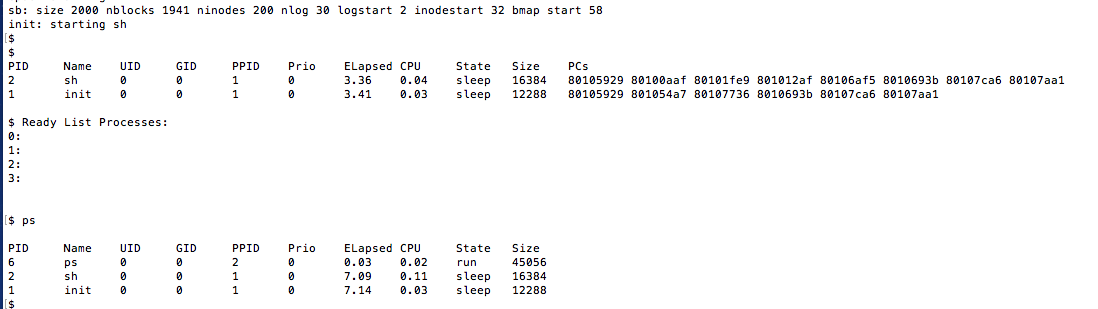
\includegraphics[width=0.6\linewidth]{demotion-start.png}
\caption{Initial output}
\label{fig:0}
\end{figure}

\begin{figure}[h]
\centering
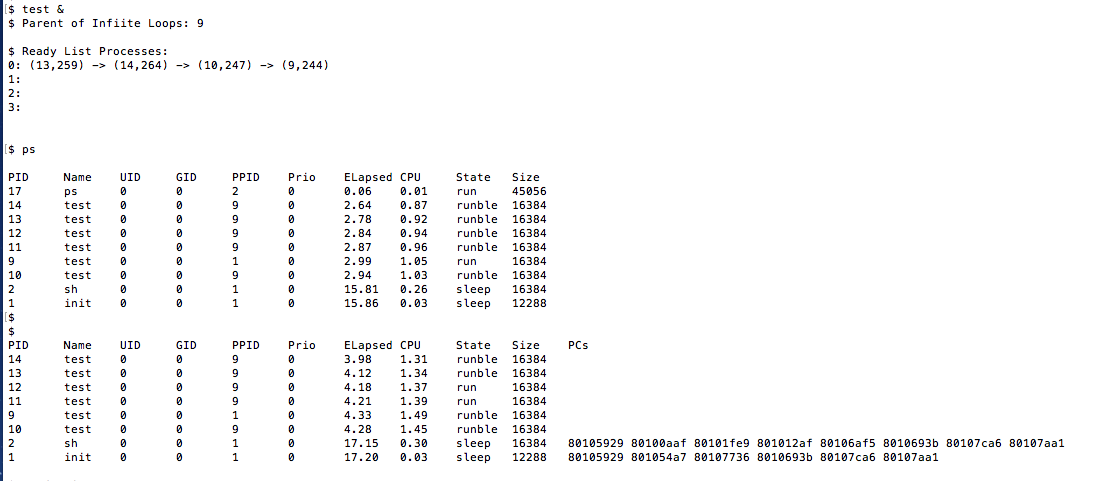
\includegraphics[width=0.8\linewidth]{demotion-0.png}
\caption{Test start, Queue 0}
\label{fig:1}
\end{figure}

\begin{figure}[h]
\centering
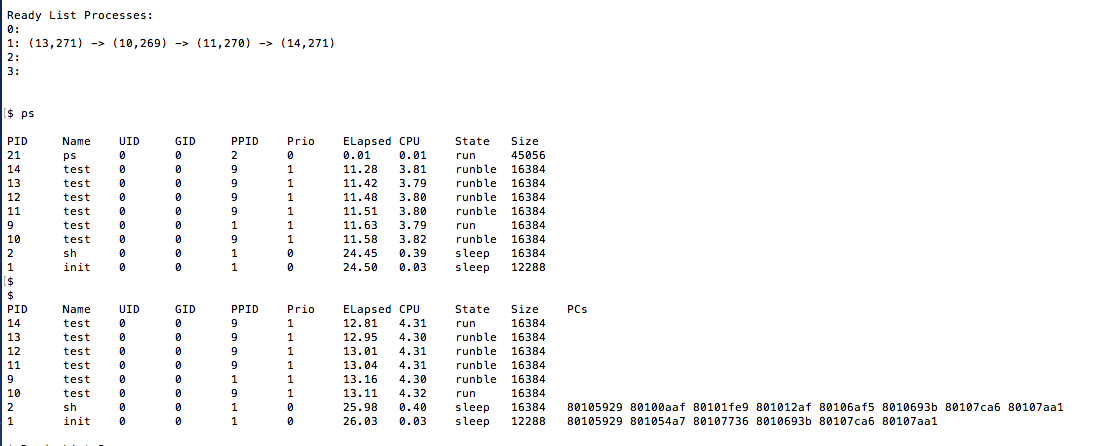
\includegraphics[width=0.8\linewidth]{demotion-1.png}
\caption{Queue 1}
\label{fig:3}
\end{figure}

\newpage

\begin{figure}[h]
\centering
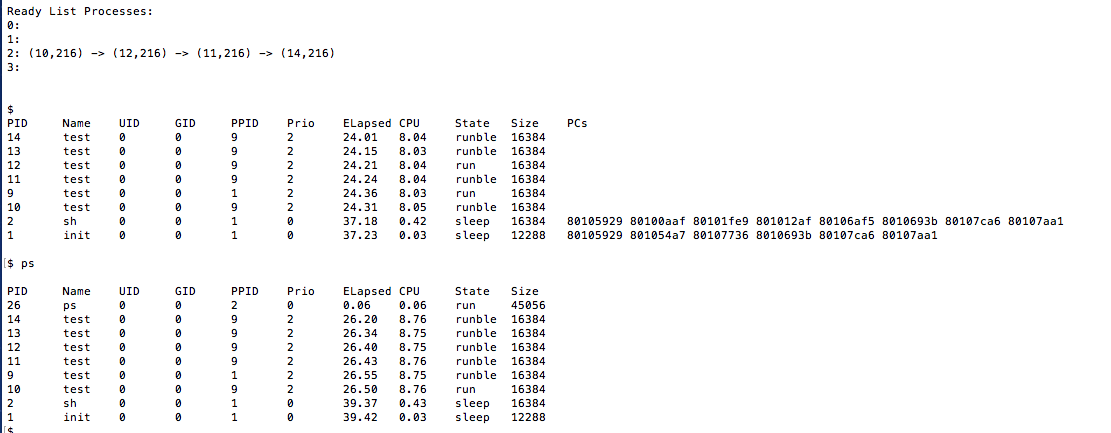
\includegraphics[width=0.8\linewidth]{demotion-2.png}
\caption{Queue 2}
\label{fig:4}
\end{figure}

\begin{figure}[h]
\centering
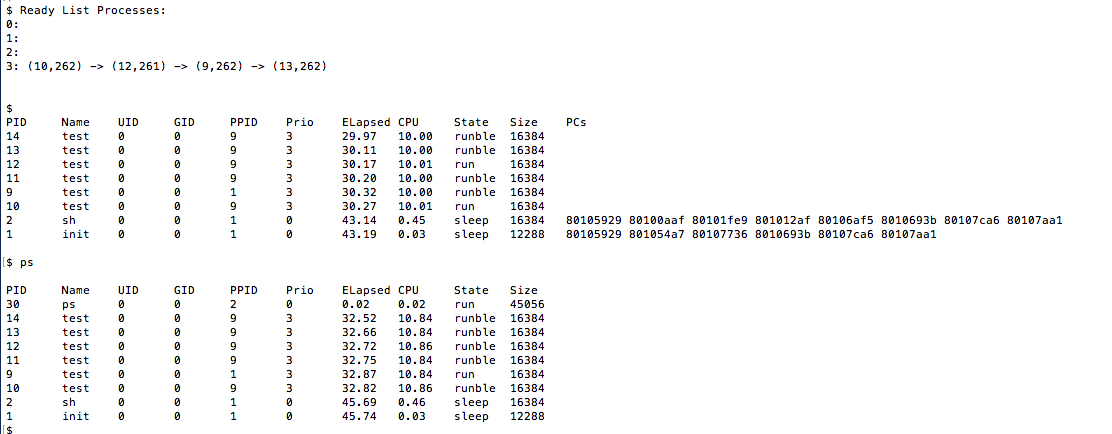
\includegraphics[width=0.6\linewidth]{demotion-3.png}
\caption{Queue 3}
\label{fig:5}
\end{figure}

\begin{figure}[h]
\centering
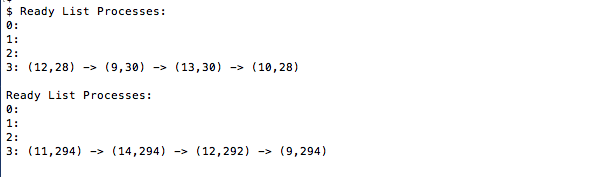
\includegraphics[width=0.6\linewidth]{demotion-4.png}
\caption{Remaining on queue 3 after budget expires}
\label{fig:5}
\end{figure}

\newpage

In figure 1, we see that initial outputs of \ctrl{p} and {\tt ps}, and process priorities match with the exception of {\tt ps}; we also see that \ctrl{r} is empty. Thus for the first step our expectations
are met. 

In figures 2-4 we see that the test begins, that all processes are demoted one queue at a time, and that our expectations for the output of \ctrl{r}, \ctrl{p}, and {\tt ps} are met. Further, at each 
priority level, \\ $(i) *$ DEFAULT\_BUDGET$ \leq CPU < (i+1) * $DEFAULT\_BUDGET indeed holds with a DEFAULT\_BUDGET of approx. 3 seconds. Thus the expectation for 
the second stage of our test have been met. 

Lastly, figure 5 shows that when a process uses up it's budget at the MAX priority, 3, that the budget is reset and the process is placed back on the MAX priority queue; this is evident by an increased budget while remaining on queue MAX.

Since all of our expectations were met at each stage of the test, this test \textbf{PASSES}.


\subsection*{Test 2 - Round Robin and Process Selection (Requirements 1, 2) }
This test will demonstrate that round robin scheduling is still enforced for a single priority level and that the MLFQ scheduler selects the first process from the highest non-empty priority queue.
To do this we will change the number of children {\tt inf\_loop()} creates to 20. We will also change the DEFAULT\_BUDGET to 2 seconds. The steps will then proceed as:
\begin{itemize}
	
	\item Execute {\tt text \&} to regain shell access. We will then hold down \ctrl{r} to get ready list info as quickly as possible; with round robin scheduling on a single priority queue we 
		expect that (similar to the Project 3 Report) with two CPUs unless the scheduler has made it through the entire list which is evident by a different budget value, 
		if some line is  A, D, E, J, H, K, P, Q, W and the next line starts 
		with a K, then K must at least be 
		followed by P, Q, W (since K didn't run P, Q and W must not have either, thus the ordering and budget for these remains) and P, Q, W must be followed by A, D, E and the two processes that \emph{were} running, 
		in some order since these ran and must have been inserted into the back of the list.
	\item We will then wait some time for all of the processes to settle down to the MAX (or lowest) priority queue. At this point we will execute {\tt text \&} again to create a new batch of processes to
		run. Since each process starts at the highest priority, these will begin at queue 0. We expect as we press \ctrl{r} repeatedly, that only process from queue 0 will be selected since $P_0>P_{MAX}$. 
		This will be evident by a changing order of queue 0 with diminishing budgets over time, and the budgets on queue MAX remaining constant.
\end{itemize}


\begin{figure}[h]
\centering
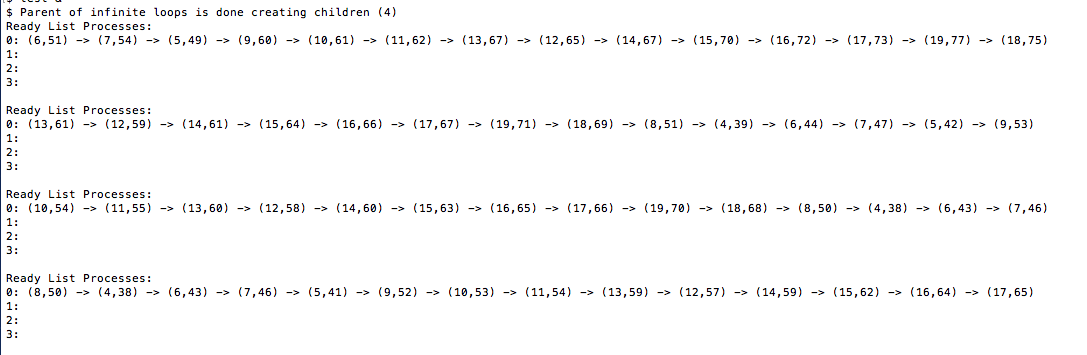
\includegraphics[width=0.8\linewidth]{rr-0.png}
\caption{Initial process batch}
\label{fig:1}
\end{figure}


\begin{figure}[h]
\centering
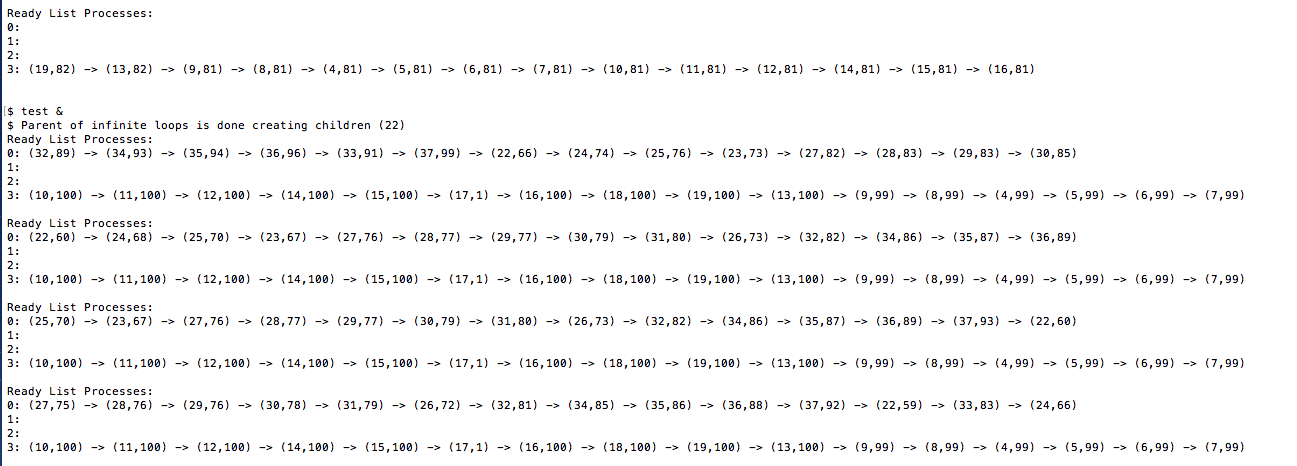
\includegraphics[width=0.8\linewidth]{rr-1.png}
\caption{Second process batch}
\label{fig:5}
\end{figure}

In figure 1 we see that in the first three outputs that the scheduler did in fact run every process on the list before \ctrl{r} was able to print again (they both use the lock); this is evident by the decreased budget on all processes between the first, second and third prints. However, the general ordering described does in fact remain. In the last output, print 4, we see (8, 50) as the head of queue 0 where on the list immediately prior, print 3, we see (8, 50) towards the tail with (4, 38), (6,43) and (7, 46) following. Since process 8 did not run between print 3 and 4, and is followed by the processes 4, 6, and 7 with unchanged budgets, we can conclude
that our expectations for round robin scheduling are in fact met.

In figure 2, we see that after the first batch had reached queue 3 (MAX) before we executed {\tt test \&} for the second time. The new batch at queue 0 is then prioritized over the last batch at queue 3 during scheduling. Again we see round robin scheduling
at queue 0 but more importantly we see that all processes on queue 3 have unchanged budgets (see PIDs to match them to batch one). Thus, figure 2 demonstrates the second stage of our test.

Because all expectations were met for each stage of this test, this test \textbf{PASSES}.


\subsection*{Test 3 - setpriority() for RUNNABLE and non-RUNNABLE processes (Requirements 5, 6) }
Here we will test that setpriority() correctly sets the priority number for both RUNNABLE and non-RUNNABLE processes and that when the priority is set for a RUNNABLE process
that the process is moved to the end of its new priority queue. To do this we will set DEAULT\_BUDGET to 100 seconds and PROMOTE\_AT\_TICKS to 100 seconds so that processes stay at their set priority for the duration of the test. The stages of this test are as follows:
	\begin{itemize}
		\item Execute {\tt test \&}. This will be set to call {\tt valid\_setpriority()} (test.c lines 198-236) which creates a batch of 15 children that will spin 
			at priority queue 0 since queue 0 
			is the inherited priority of any created processes and the DEAULT\_BUDGET is greater than the time we will allow them to spin.
		
		\item The parent will then notify us it completed the first stage and create 5 more processes, where it will set the priority of these  5 children priority to MAX. Because the first stage filled
			queue 0 with spinning processes, the call to {\tt valid\_setpriority()} with a valid PID and priority will likely occur before the child first runs. {\tt valid\_setpriority()} 
			will then take the child off queue 0
			and place it upon queue MAX. The parent will notify us of it's success (through the return code of {\tt valid\_setpriority()}) and sleep for a moment. At this point we will press \ctrl{r}
			which was demonstrated to be correct in Test 1. Here we expect since {\tt valid\_setpriority()} was successful, and the child likely did not run, that it will be at the \emph{end} of queue MAX
			with a full budget of 10,000.
		
		\item The parent will then kill all children it created thus far. 
		
		\item Lastly the parent will create 3 more children who will immediately sleep. The parent will print the PID of the created child, sleep for a few seconds to allow the children to 
			get to the SLEEPING state and let us press \ctrl{p}. At this point we expect to see it in the SLEEPING state with priority 0. The parent will then call {\tt valid\_setpriority(childPID, MAX);}
			after being notified we will press \ctrl{p} again and now expect to the the priority of this child set to MAX - or 3 in this case.
	\end{itemize}
	
\begin{figure}[h]
\centering
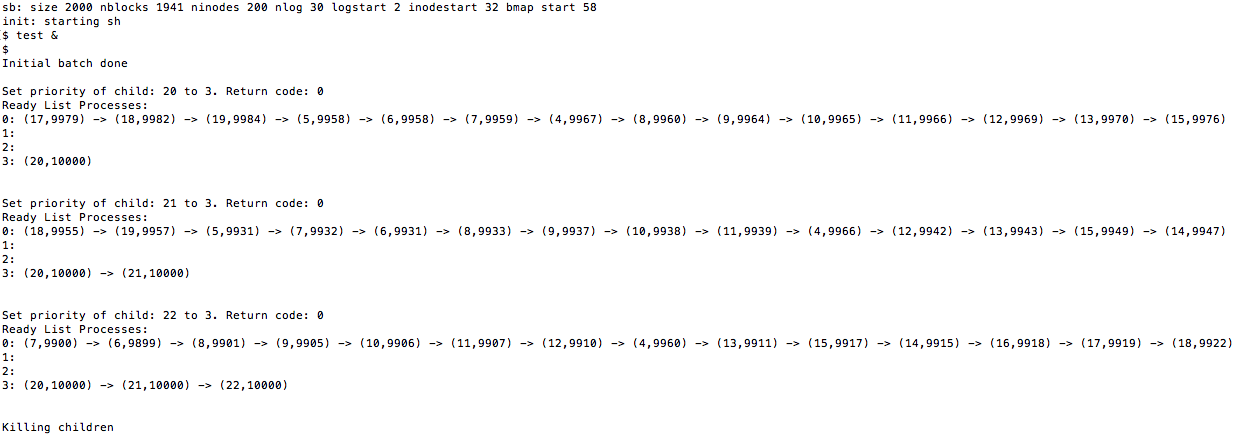
\includegraphics[width=0.8\linewidth]{prio-runnable.png}
\caption{Runnable priorityset()}
\label{fig:5}
\end{figure}

\pagebreak

\begin{figure}[h]
\centering
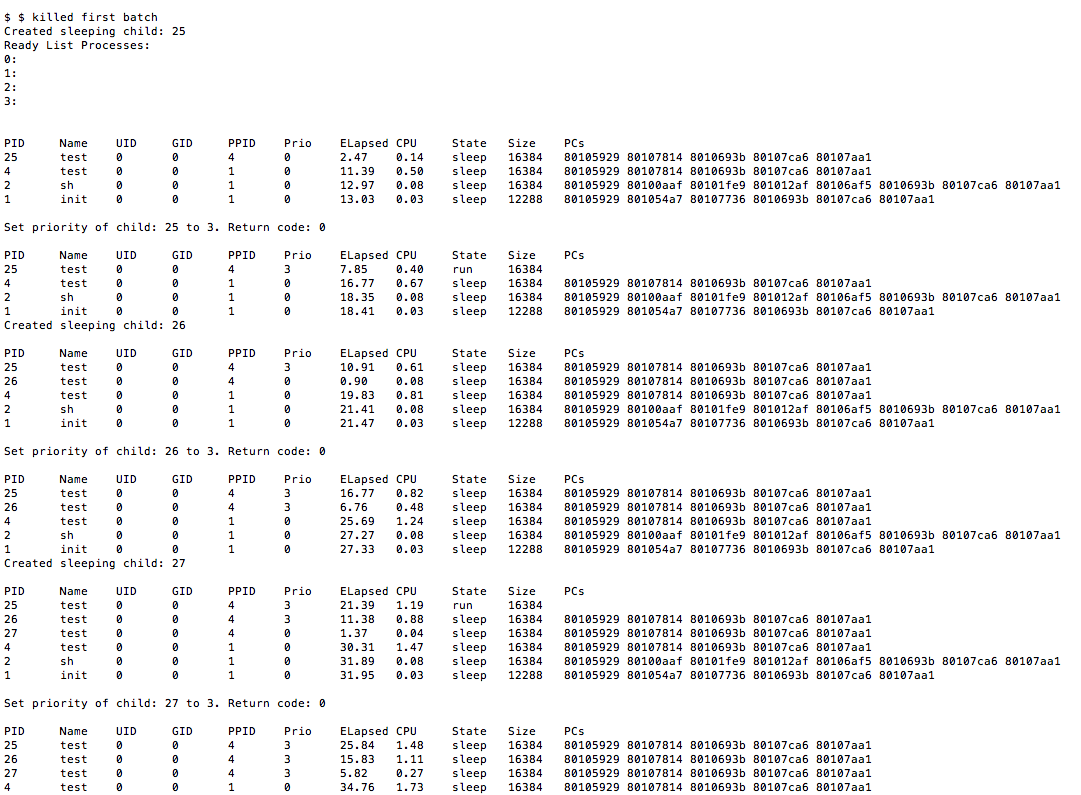
\includegraphics[width=0.8\linewidth]{prio-nonrunnable.png}
\caption{Sleeping (non-runnable) priorityset()}
\label{fig:5}
\end{figure}



In figure 8 we see that for each child created, after the parent sets its priority that the child is placed at the end of the MAX queue \emph{and} that
the return code is 0 - indicating success. Thus our expectations for this stage of the test are met.

In figure 9, we see that all the children are in fact killed - reflected by \ctrl{p} which was demonstrated as correct in Test 1. We also see that the child
makes it to the SLEEPING state with priority 0 before {\tt setpriority()} is called and that after {\tt setpriority()} is called it has the correct MAX priority
and it is still in sleeping. The return code is 0 in all cases. Thus, our expectations for this stage of the test are met.

Because our expectations were met at each stage of the test, this test \textbf{PASSES}

\subsection*{Test 4 - Priority Promotion (Requirements 3) }
Here we will test that the priority promotion component of the MLFQ works as expected. To do this we will set DEAULT\_BUDGET to 100 seconds and PROMOTE\_AT\_TICKS to 5 seconds then simply run {\tt prioritypromotion()} (test.c lines 276-304) through executing {\tt test}. 
\begin{itemize}
	\item The parent will create 10 spinning children that will remain on queue 0.
	
	\item The function will then create 10
		spinning children and 
		place them at queue MAX, or 3 by calling {\tt setpriority()} - demonstrated in Test 3. After being notified that the low priority children are all created we will press \ctrl{r} approximately every 5 seconds and expect to see all processes at queue 0, remain at queue 0 but have their budget reset to 10000. Because we likely cannot press \ctrl{r} before a process runs
		again after having its budget reset, we expect each budget to remain between 9000-10000 even though each process has run for more than one 
		second.  
		We also expect the processes at queue MAX to increase one priority queue after each promotion so we will see them on queue 3, 2, 1, then 0.
		Additionally we expect to see that the exact order of the queue remains - this will be our best demonstration that one queue is appended to the end of the next highest queue. Their budgets wont change since they do not run; this is in accordance with the
		MLFQ algorithm outlined in the requirements section and as demonstrated by Test 2. When the lower priority children are promoted to priority queue 0, we expect they will be appended to the end. 
		However, the short-comming of this test is that we will not be able to perfectly identify this moment in time. Thus, we expect that if the originally lower
		priority processes are not at the end, that their budget will not be 10000 since they must have run. Due to the round robin scheduling demonstrated 
		in test 2, the general ordering should remain.
\end{itemize}

\begin{figure}[h]
\centering
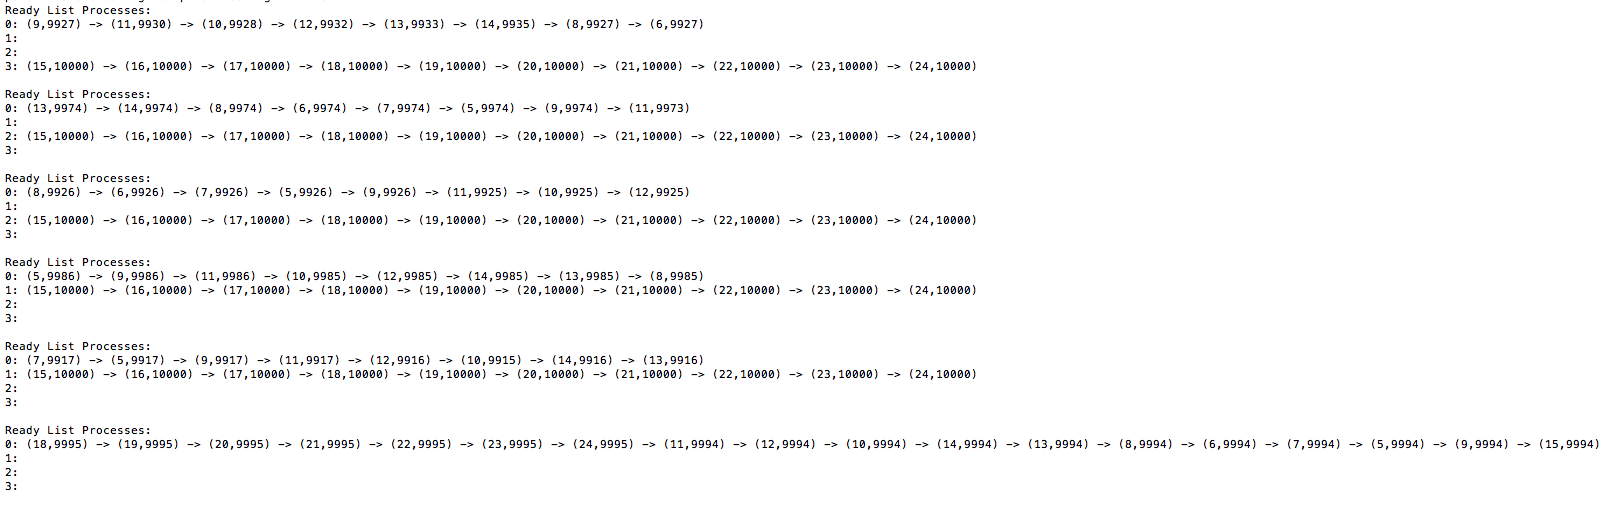
\includegraphics[width=1\linewidth]{promotion.png}
\caption{Priority Promition}
\label{fig:5}
\end{figure}

In figure 11 we see that we were not precise in our pressing of \ctrl{r} every 5 seconds, so there are sometimes two displays between promotions. 
However we do see that the budget of all processes on queue 0 are always between 9000 and 10000, and that the budgets on the lower priority queue do not change. Demonstrating the budget reset of the priority boost, between \ctrl{r} print 3 and 4 we see process 8 on queue 0 has an increased budget! Thus this expectation of stage 2 of the test is met. We also see that the lower priority queue moves from 3 to 2 to 1 to 0 with the exact ordering retained, as expected and that once it reaches queue 0 its general ordering remains. Although these processes made it to the head of the queue, their budget is less than 10000 and thus have since run, meaning we could not see them at the end of queue 0 immediately following the priority reset. The limitations of this have been acknowledged.

Since our expectations for each stage of this test were met, this test \textbf{PASSES}.

\subsection*{Test 5 - Invalid setpriority() calls (Requirements 7, 8) }
This test will demonstrate that setpriority() calls with invalid arguments will return an error code, and not update the priority of the PID given.
To do this we will add {\tt invalid\_priorityset()} to the user program {\tt test} (test.c lines 256-274). When will then:

\begin{itemize}
	\item Begin by executing {\tt test \&} and pressing \ctrl{p}, while it initially sleeps, to see all active process information.

	\item 
		When {\tt test} wakes after 2 seconds, {\tt invalid\_priorityset()} will then call {\tt priorityset(PID, PRIORITY)} with PIDs -1, 1000, and 9999 and a priority of MAX. 
		Since we know by virtue of the code, that PIDs
		are assigned in increasing order and that only sh and initproc are running at boot, all of these PIDs are invalid. This is confirmed by the \ctrl{p} output. We also know that MAX is a valid priority so that the failure of this call is strictly due to the PID  being invalid.
		Thus when the process prints the values attempted to be assigned and the return code, we expect a return code of -1. 

	\item Next, the {\tt test} will attempt to assign invalid priorities for the process init which has a PID of 1, confirmed by \ctrl{p}, printing its attempts and the return codes. The invalid priorities given will be MAX+1 and MAX+2. After which, \ctrl{p} will be pressed. We expect that {\tt test} will have printed -1 for all return codes, and that the priority for init will remain unchanged. 
\end{itemize}

\begin{figure}[h]
\centering
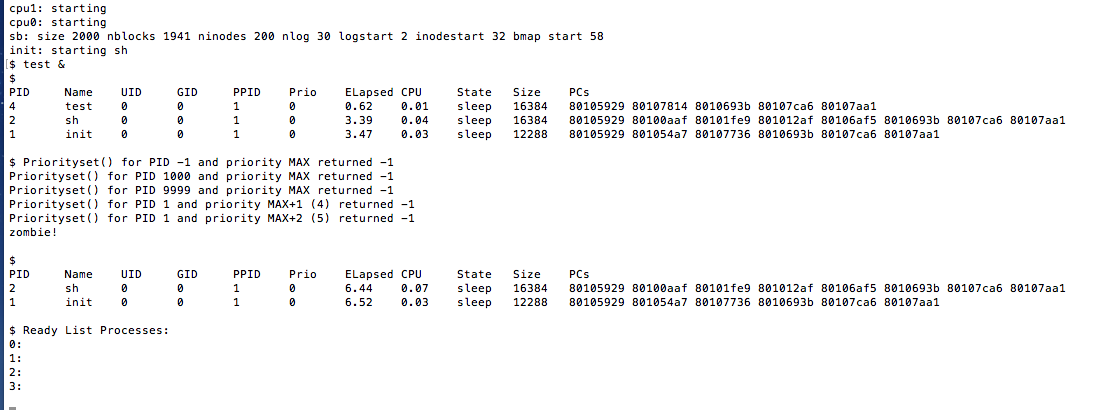
\includegraphics[width=0.8\linewidth]{invalid-priority.png}
\caption{Invalid setpriority() calls}
\label{fig:5}
\end{figure}
 
 As expected, all calls to setpriority() returned -1 indicating failure. PIDs -1, 1000, and 9999 did not exist on \ctrl{p}. Init indeed had a PID of 1 but its priority did not change. Note the ready list output indicates MAX was 3 and the calls to change the priority of init were 4 and 5 respectively.
 
 Since all our expectations for this test were met, this test \textbf{PASSES}. 
 
\subsection*{Test 6 - MLFQ with generic MAX (Requirement 9) }
This test will demonstrate that the new MLFQ will operate as expected with a generic MAX value. To do this we will change MAX to 1, 3, and
7 with DEFAULT\_BUDGET set to 100 seconds and TICKS\_TO\_PROMOTE set to 5 seconds- recompiling each time. 

We will then invoke {\tt test \&} to regain shell control, where {\tt test} will execute the function {\tt prioritypromotion()} described in 
Test 4. Since {\tt prioritypromotion()} relied on MAX to set the lower priority values, our expectations for the process promotion with a MAX of 1, 3, and 7 will
be the same as in Test 4 (please reference Test 4 for outline of expectations). An additional expectation will be that the MAX queue is numbered corresponding to what MAX is defined as in the compilation (i.e. 1, 3, and 7 respectively).

\begin{figure}[h]
\centering
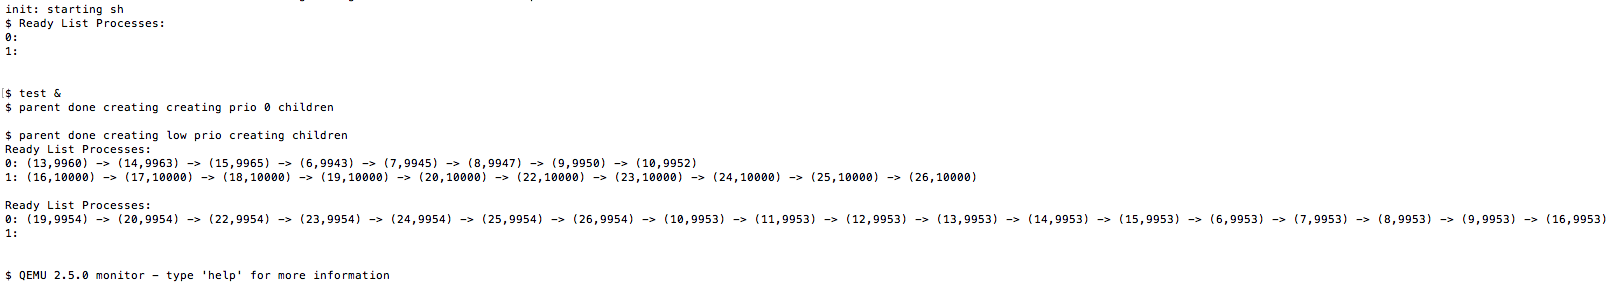
\includegraphics[width=1\linewidth]{max-1.png}
\caption{MAX of 1}
\label{fig:5}
\end{figure}


\begin{figure}[h]
\centering
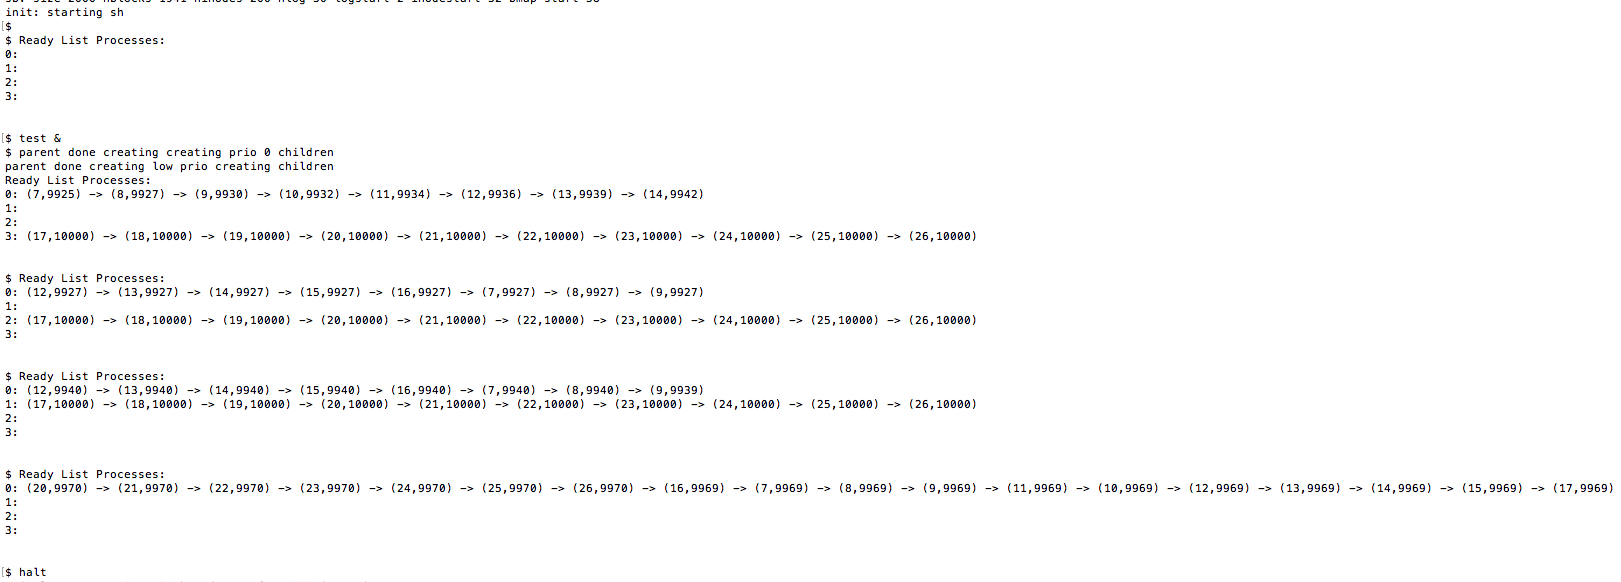
\includegraphics[width=0.9\linewidth]{max-3.png}
\caption{MAX of 3}
\label{fig:5}
\end{figure}
\pagebreak

\begin{figure}[h]
\centering
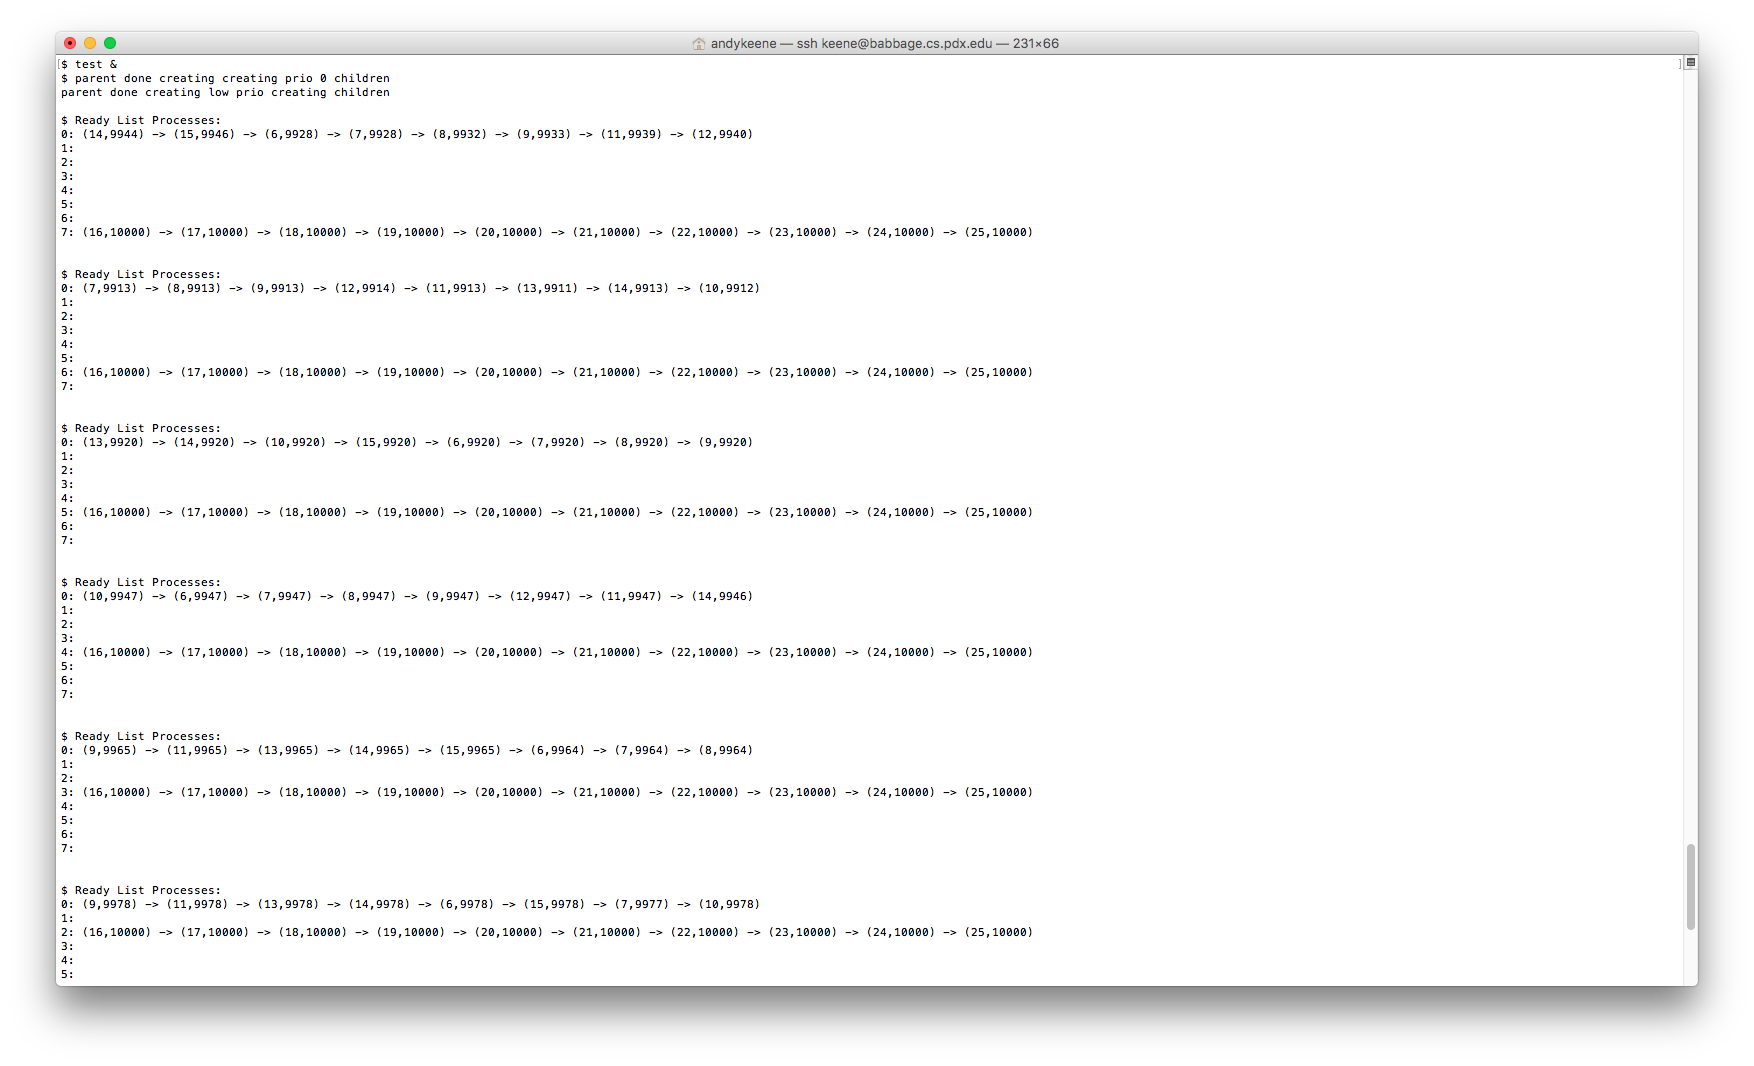
\includegraphics[width=0.8\linewidth]{max-7a.png}
\caption{MAX of 7, part 1}
\label{fig:5}
\end{figure}

\begin{figure}[h]
\centering
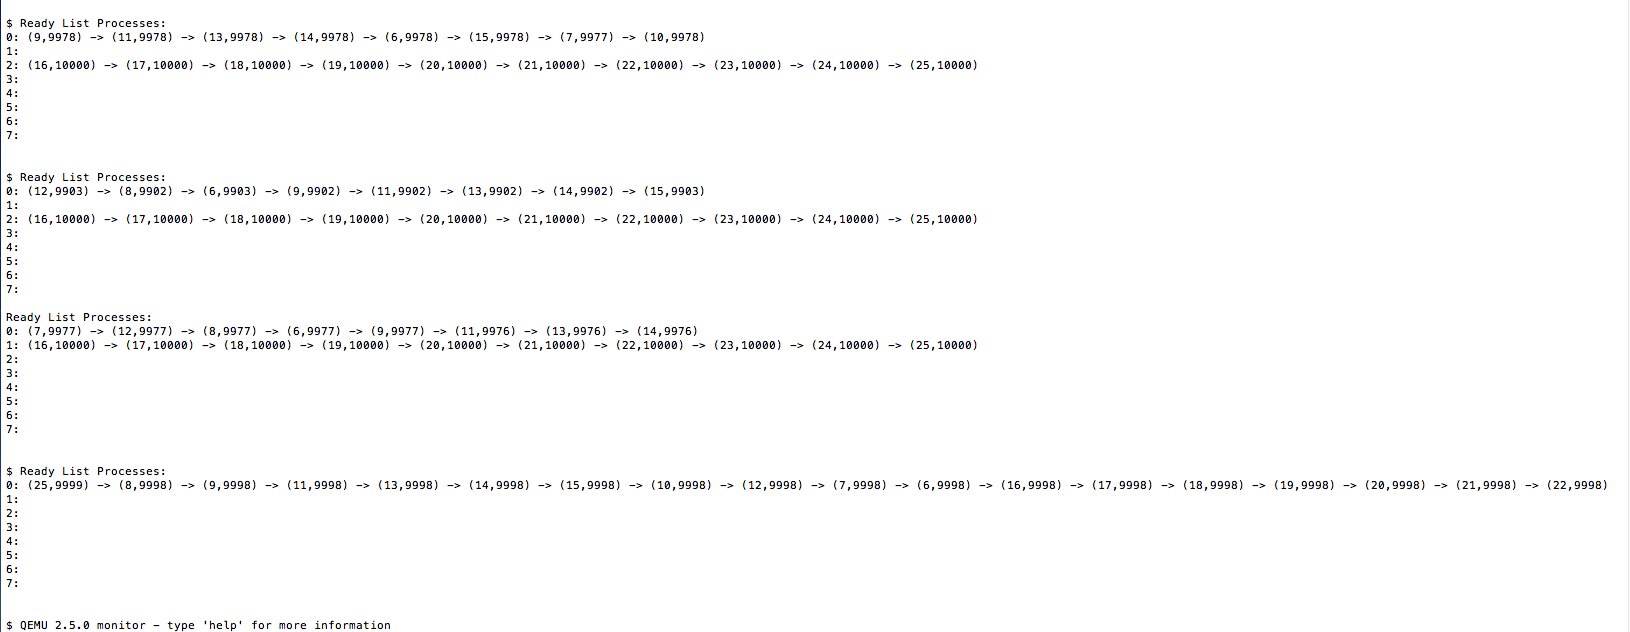
\includegraphics[width=0.8\linewidth]{max-7b.png}
\caption{Max of 7, part 2}
\label{fig:5}
\end{figure}

\pagebreak
In figures 13-15 demonstrating priority promotion for MAXes of 1, 3, and 7 we see that each \ctrl{r} display at approximately 5 second intervals shows: a budget reset 
evident on the top-most priority queue; a promotion for the lower priority processes from queue MAX, MAX-1,..., 0; and that the lower priority processes are appended to queue 0 evident by
the retention of general ordering with a non-full budget (acknowledged limitation of Test 4). Thus all expectations for priority promotion with MAX set to 1, 3, and 7, are met.
Because all expectations for this test were met, this test \textbf{PASSES}

Further, because all tests passed we can conclude that the corresponding requirements 1-12 have been fulfilled.

\end{document}




